%%% Copyright (C) 2017 Vincent Goulet
%%%
%%% Ce fichier fait partie du projet «Programmer avec R»
%%% http://github.com/vigou3/programmer-avec-r
%%%
%%% Cette création est mise à disposition selon le contrat
%%% Attribution-Partage dans les mêmes conditions 4.0
%%% International de Creative Commons.
%%% http://creativecommons.org/licenses/by-sa/4.0/

\chapter{Éléments d'informatique pour programmeurs}
\label{chap:informatique}

Intro du chapitre

\section{Bref historique des langages de programmation}
\label{sec:informatique:historique}

Ada Lovelace (1815--1852) est généralement reconnue comme la première
auteure d'un algorithme et de ce que l'on appelle aujourd'hui un
programme informatique. C'est en son honneur qu'été nommé le langage
Ada conçu en réponse à un cahier de charges du département de la
Défense des États-Unis au début des années 1980.

Franchissons d'un bond les premiers jours de l'informatique et de la
programmation\footnote{%
  Les lecteurs intéressés à en apprendre davantage sur le sujet
  pourront débuter par les entrées de Wikipedia
  (\link{https://fr.wikipedia.org/wiki/Histoire_des_langages_de_programmation}{français},
  \link{https://en.wikipedia.org/wiki/History_of_programming_languages}{anglais}).} %
pour arriver aux ordinateurs électriques modernes, dans les années
1940. On programme alors généralement ceux-ci en \emph{assembleur}, un
langage de très bas niveau facilement interprétable par la machine,
mais difficile à lire par des humains; voir la
\autoref{fig:informatique:assembleur}.

\begin{figure}
  \centering
  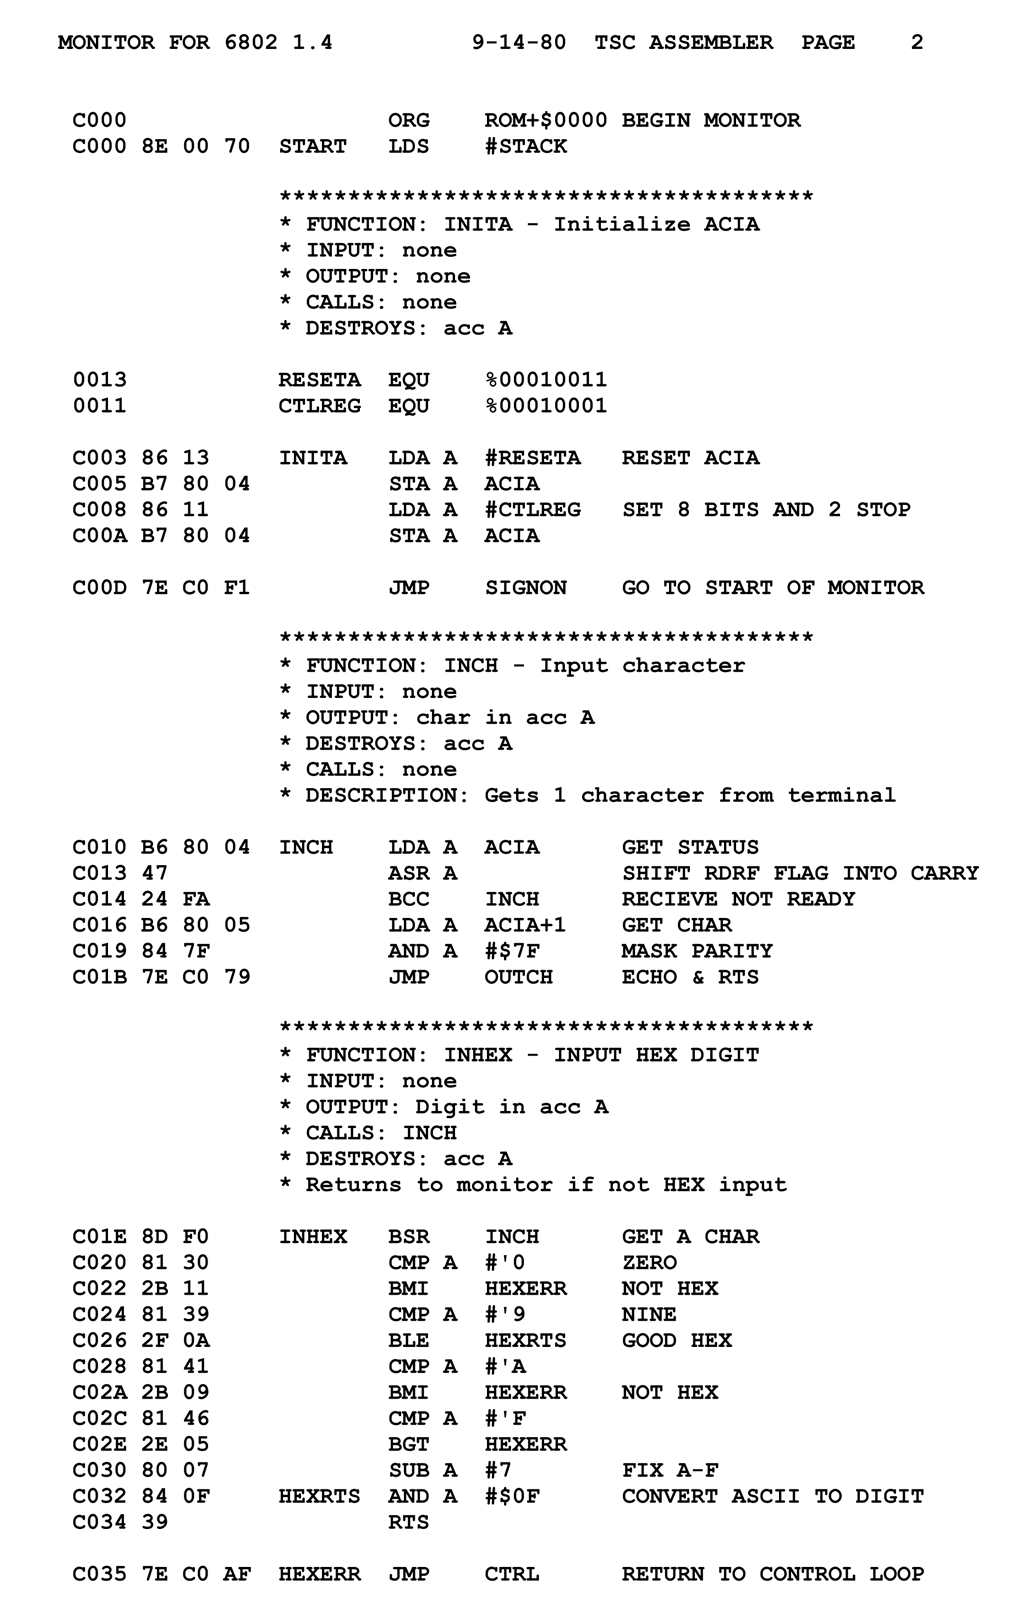
\includegraphics[trim=0 475 0 0, clip=true]{Motorola_6800_Assembly_Language.png}
  \caption[Programme assembleur pour un microprocesseur 8~bits
  Motorola 6800.]{Extrait d'un programme en assembleur pour un
    microprocesseur 8~bits Motorola 6800. Source:
    \link{https://commons.wikimedia.org/wiki/File\%3AMotorola_6800_Assembly_Language.png}{Wikimedia Commons}}
  \label{fig:informatique:assembleur}
\end{figure}

Les premiers langages créés pour transmettre des instructions à un
ordinateur apparaissent dans les années 1950. Ils sont à l'origine
intimement liés à l'architecture d'un ordinateur: à chaque type
d'ordinateur son langage de programmation. Certaines contraintes ---
ou exigences --- des langages de l'époque proviennent aussi du support
physique alors utilisé pour stocker les programmes: les cartes
perforées.

En 1954, l'ingénieur de IBM John Backus publie les spécifications du
langage FORTRAN (\emph{FORmula TRANslating System}). Le premier
compilateur voit le jour deux ans plus tard. Fortran (avec des
minuscules à partir de 1977) deviendra rapidement le langage standard
dans le calcul scientifique. Plus d'un demi-siècle plus tard, son
empreinte demeure importante, notamment grâce aux bibliothèques
d'algèbre linéaire BLAS\footnote{%
  \emph{Basic Linear Algebra Subprograms};
  \link{http://www.netlib.org/blas}{}.} %
et LAPACK\footnote{%
  \emph{Linear Algebra PACKage};
  \link{http://www.netlib.org/lapack}{}.} %
auxquelles ont recours la plupart des progiciels scientifiques, dont
R.

\begin{figure}[t]
  \notebox{Dans le très recommandable film Les figures de l'ombre
    (\emph{Hidden Figures}, 2016), une des héroïnes entreprend de
    s'attaquer à la programmation des nouveaux ordinateurs de la NASA.
    On peut alors voir qu'elle apprend le Fortran.}
\end{figure}

Le deuxième langage le plus ancien toujours largement diffusé est Lisp
(\emph{LISt Processing}). Créé par John McCarthy en 1958 en tant
que modèle pratique pour représenter des programmes, le Lisp est
devenu le langage de choix pour la recherche et les applications en
intelligence artificielle. Il se distingue en outre par une syntaxe
simple en notation préfixée (voir encadré), le support pour la
programmation fonctionnelle (\autoref{sec:informatique:paradigmes}) et
la faculté de manipuler le code source en tant que structure de
données. Le terme Lisp désigne aujourd'hui une famille de langages
comprenant de nombreux dialectes, dont Common Lisp, Scheme et Emacs
Lisp.

\begin{figure}[t]
  \setlength{\FrameRule}{1pt}
  \begin{emphbox}{\mdseries Notations infixée, préfixée et suffixée}
    Les notations infixée (\emph{infix}), préfixée (\emph{prefix}) et
    suffixée (\emph{postfix}) sont trois manières différentes, mais
    équivalentes, d'écrire des expressions en mathématiques ou en
    programmation.

    Par exemple, l'opération d'addition de deux opérandes $x$ et $y$
    s'écrit en notation infixée
\begin{lstlisting}[backgroundcolor=\color{codebg}]
x + y
\end{lstlisting}
    En notation préfixée, aussi appelée notation polonaise,
    l'opérateur est placé \emph{avant} les opérandes:
\begin{lstlisting}[backgroundcolor=\color{codebg}]
+ x y
\end{lstlisting}
    On l'aura compris, en notation suffixée, ou notation polonaise
    inversée, l'opérateur apparait \emph{après} les opérandes:
\begin{lstlisting}[backgroundcolor=\color{codebg}]
x y +
\end{lstlisting}
    Nous sommes davantage habitués à lire la notation infixée, quoique
    la notation préfixée nous soit familière pour les opérateurs à un
    seul opérande (comme la négation) ou pour les appels de fonctions.
    La notation suffixée n'a jamais recours aux parenthèses.

    La compagnie HP commercialise de très prisées calculatrices
    scientifiques utilisant la notation suffixée (libellées RPN pour
    \emph{Reverse Polish Notation}) depuis 1972.
  \end{emphbox}
\end{figure}

Le Lisp est entouré d'une aura de beauté et d'élégance dont peu
d'autres langages peuvent se targuer. Citons Eric Raymond
dans
\link{http://www.catb.org/esr/faqs/hacker-howto.html}{\emph{How to
    Become a Hacker}}:
\begin{quote}
  Il faut apprendre le Lisp pour l'extraordinaire expérience d'éveil
  que procure le fait de finalement le comprendre; cette expérience
  fera de vous un meilleur programmeur pour toujours, même si vous
  n'avez plus vraiment à utiliser le Lisp. (Traduction libre)
\end{quote}

Pour illustrer encore davantage la place toute particulière qu'occupe
le Lisp en programmation, mentionnons également l'aphorisme selon
lequel «ceux qui ne connaissent pas le Lisp sont condamnés à le
réinventer», d'une certaine façon la version courte de la célèbre
\link{https://en.wikipedia.org/wiki/Greenspun\%27s_tenth_rule}{\emph{Greenspun's
    tenth rule of programming}}\footnote{%
  Fait à noter, il n'y a pas d'autres lois que la dixième, de
  l'\link{http://philip.greenspun.com/bboard/q-and-a-fetch-msg?msg_id=000tgU}{aveu
    même de l'auteur}.}: %
\begin{quote}
  Tout programme en C ou en Fortran suffisamment complexe contient
  une implémentation mal spécifiée, pleine de bogues et lente de la
  moitié de Common Lisp. (Traduction libre)
\end{quote}

Complétons notre tour d'horizon des langages développés dans les
années 1950 et toujours en usage de nos jours par COBOL (\emph{COmmon
  Business Oriented Language}). Ce langage spécialisé dans les
applications de gestion a été créé en 1959 par un comité formé pour
proposer un langage commun pour l'administration américaine. La
légende urbaine veut que les programmeurs COBOL soient comparativement
très bien rémunérés aujourd'hui sous l'effet combiné de leur rareté et
de l'importance opérationnelle des applications qu'ils doivent
maintenir.

Dès la fin de la décennie 1950, un comité de scientifiques se réunit à
Zurich pour concevoir ce que l'on voudrait voir devenir le langage de
programmation standard. De ces rencontres naîtra Algol
(\emph{ALGorithmic Oriented Language}) en 1958. Comme la plupart des
tentatives de définition d'un standard, c'est un échec: le langage est
populaire dans les milieux académiques, mais restera peu utilisé dans
les applications commerciales. Néanmoins, on doit à Algol plusieurs
innovations importantes, de telle sorte qu'un grand nombre des
langages qui verront le jour par la suite seront considérés comme ses
descendants. \citet{Hoare:1973} a d'ailleurs cette jolie formule:
«Voici un langage très en avance de son temps, il n'a pas seulement
été une amélioration de ses prédécesseurs mais aussi une amélioration
de presque tous ses successeurs.»

\begin{figure}[t]
  \centering
  \begin{minipage}{0.9\linewidth}
    \setkeys{Gin}{width=\textwidth}
    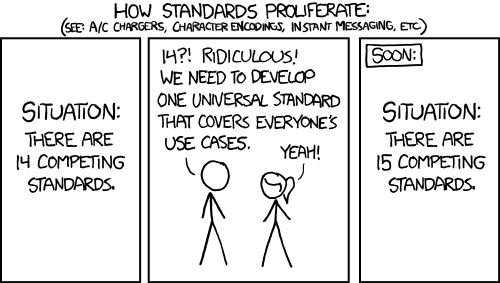
\includegraphics{standards} \\
    \footnotesize\sffamily%
    Tiré de \href{http://xkcd.com/927/}{XKCD.com}
  \end{minipage}
\end{figure}

APL (1962) longtemps un langage très prisé par les actuaires; probablement
encore du code APL dans certaines compagnies d'assurance; inspiration
pour S et R; continue sa vie aujourd'hui surtout sous J.



C Kernighan et Ritchie, Bell Labs -> John Chambers et S; Unix;
toujours beaucoup utilisé pour le calcul numérique intensif; évolution
vers C++

Python (1991)
\url{https://en.wikipedia.org/wiki/Python_(programming_language)}







\section{Syntaxe et sémantique}
\label{sec:informatique:syntaxe}

\section{Paradigmes de programmation}
\label{sec:informatique:paradigmes}

\section{Systèmes d'exploitation}
\label{sec:informatique:os}



%%% Local Variables:
%%% mode: latex
%%% TeX-engine: xetex
%%% TeX-master: "programmer-avec-r"
%%% End:
